% !TEX encoding = UTF-8 Unicode
\documentclass[a4paper]{article}

\usepackage{color}
\usepackage{url}
\usepackage[T2A]{fontenc} % enable Cyrillic fonts
\usepackage[utf8]{inputenc} % make weird characters work



\usepackage{graphicx}
\graphicspath{ {./slike/} }

\usepackage[english,serbian]{babel}
%\usepackage[english,serbianc]{babel} %ukljuciti babel sa ovim opcijama, umesto gornjim, ukoliko se koristi cirilica

\usepackage[unicode]{hyperref}
\hypersetup{colorlinks,citecolor=green,filecolor=green,linkcolor=blue,urlcolor=blue}

\usepackage{listings}

%\newtheorem{primer}{Пример}[section] %ćirilični primer
\newtheorem{primer}{Primer}[section]

\definecolor{mygreen}{rgb}{0,0.6,0}
\definecolor{mygray}{rgb}{0.5,0.5,0.5}
\definecolor{mymauve}{rgb}{0.58,0,0.82}

\lstset{ 
  backgroundcolor=\color{white},   % choose the background color; you must add \usepackage{color} or \usepackage{xcolor}; should come as last argument
  basicstyle=\scriptsize\ttfamily,        % the size of the fonts that are used for the code
  breakatwhitespace=false,         % sets if automatic breaks should only happen at whitespace
  breaklines=true,                 % sets automatic line breaking
  captionpos=b,                    % sets the caption-position to bottom
  commentstyle=\color{mygreen},    % comment style
  deletekeywords={...},            % if you want to delete keywords from the given language
  escapeinside={\%*}{*)},          % if you want to add LaTeX within your code
  extendedchars=true,              % lets you use non-ASCII characters; for 8-bits encodings only, does not work with UTF-8
  firstnumber=1000,                % start line enumeration with line 1000
  frame=single,	                   % adds a frame around the code
  keepspaces=true,                 % keeps spaces in text, useful for keeping indentation of code (possibly needs columns=flexible)
  keywordstyle=\color{blue},       % keyword style
  language=Python,                 % the language of the code
  morekeywords={*,...},            % if you want to add more keywords to the set
  numbers=left,                    % where to put the line-numbers; possible values are (none, left, right)
  numbersep=5pt,                   % how far the line-numbers are from the code
  numberstyle=\tiny\color{mygray}, % the style that is used for the line-numbers
  rulecolor=\color{black},         % if not set, the frame-color may be changed on line-breaks within not-black text (e.g. comments (green here))
  showspaces=false,                % show spaces everywhere adding particular underscores; it overrides 'showstringspaces'
  showstringspaces=false,          % underline spaces within strings only
  showtabs=false,                  % show tabs within strings adding particular underscores
  stepnumber=2,                    % the step between two line-numbers. If it's 1, each line will be numbered
  stringstyle=\color{mymauve},     % string literal style
  tabsize=2,	                   % sets default tabsize to 2 spaces
  title=\lstname                   % show the filename of files included with \lstinputlisting; also try caption instead of title
}




% Dodao Petar
\usepackage[]{algorithm2e}
\usepackage{subcaption}
%%%%%

\begin{document}

\title{Primene memetskog algoritma\\ \small{Seminarski rad u okviru kursa\\Metodologija stručnog i naučnog rada\\ Matematički fakultet}}

\author{Bogićević Marica, Karanović Boris, Košanin Petar, Šašić Filip\\ kontakt email prvog, drugog, trećeg, četvrtog autora}

%\date{9.~april 2015.}

\maketitle

\abstract{
TODO}

\tableofcontents

\newpage

\section{Uvod}
\label{sec:uvod}

TODO



\section{Primene memetskog algoritma}
\label{sec:primene_memetskog_algoritma}
TODO


\subsection{Problem bojenja grafa}
\label{sec:bojenje_grafa}
Neka je zadat neusmeren graf $G = (V, E)$, gde je $V$ skup čvorova, a $E$ skup grana tog grafa. 
Bojenje grafa $G$ predstavlja problem dodeljivanja ''boja'' elementima grafa\footnote{Problem isključivo zavisi od \textit{broja} boja, a ne od konkretnih boja.}. 
Bojenje čvorova je pridruživanje po jedne boje svakom čvoru grafa $G$. 
Dodavanjem ograničenja maksimalnog broja boja, dobijamo problem k-bojenja grafa. \textit{Ispravno k-bojenje grafa} $G$ je ono za koje ne postoje dva susedna čvora\footnote{Dva čvora su susedna, ako postoji grana koja ih povezuje.} koji su obojeni istom bojom. 
Drugim rečima, ispravno k-bojenje grafa deli čvorove skupa $V$ u $k$ nezavisnih podskupova, pri čemu jedan taj podskup čine nesusedni čvorovi, obojeni istom bojom.


\begin{figure}[h!]
	\centering

	\begin{subfigure}[normla]{0.3\textwidth}
		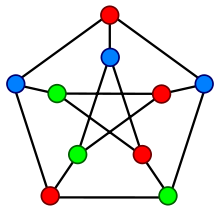
\includegraphics[scale=0.3]{bojene_grafa1}
		\caption{Primer ispravnog bojenja čvorova grafa}
		\label{bojenje_grafa1}
	\end{subfigure}
	~
	\begin{subfigure}[normla]{0.3\textwidth}
		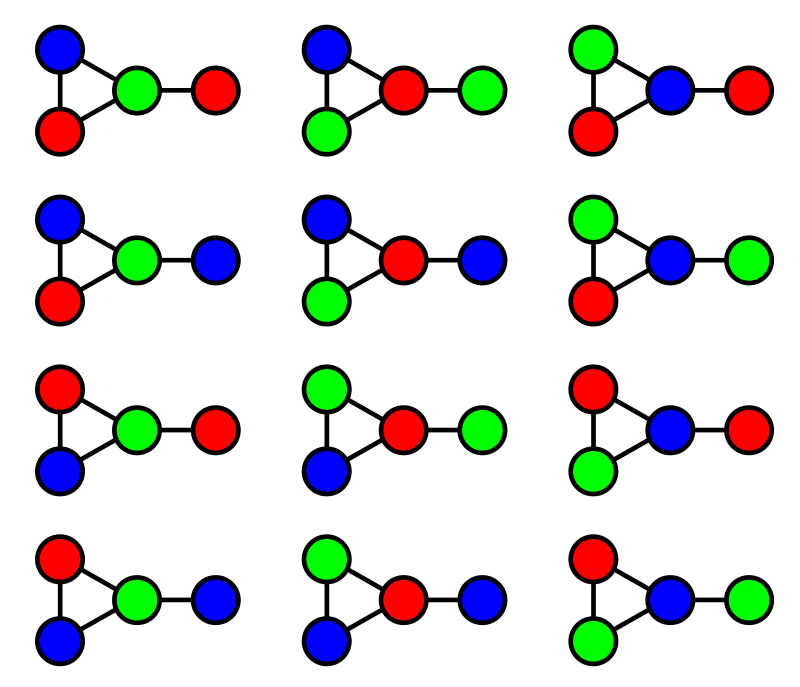
\includegraphics[scale=0.1]{bojenje_grafa2}
		\caption{Različita ispravna bojenja čvorova grafa}
		\label{bojenje_grafa2}
	\end{subfigure}
		\caption{Slika (a) prikazuje ispravno 3-bojenje Pitersonovog grafa, dok na slici (b) prikazano je 12 različitih načina 3-bojanja grafa. Izvor slika \cite{graph_coloring} }
\label{bojene_grafa}
\end{figure}

Pored svoje teoretske značajnosti kao NP-kompletan problem \cite{zivkovic_algoritmi}, bojenje grafa nalazi primenu u praksi, a neki od problema koji se svode na bojenje grafa su alokacija registara, izrada rasporeda, raspoređivanje komunikacije satelita \cite{lu2010memetic}.

Rešavanje problema bojenja grafa može se predstaviti preko rešavanja serije problema k-bojenja grafa \cite{galinier1999hybrid}. 
Naime, rešavanje problema počinje sa inicijalnom vrednošću $k \leq |V|$. 
Ako se nađe rešenje za $k$, vrednost $k$ postavljamo na $k-1$, i ponavljamo proces sve dok ne naiđemo na $k$ za koje ne postoji rešenje.

U nastavku biće opisane tri varijacije memetskog algoritma za rešavanje problema bojenja grafa. 

\subsubsection{HCA}
U radu \cite{galinier1999hybrid}, predložen je HCA(eng. Hybrid Coloring Algorithm) za rešavanje problema bojenja grafa.
HCA čine 4 glavne komponente, \textit{generator inicijalne populacije}, \textit{operator ukrštanja}, \textit{lokalna pretraga}, i \textit{pravila ažuriranja populacije}.

Jednu jedinku populacije čini podela skupa $V$ na $k$  disjunktnih podskupova $\{V_1, V_2, ...., V_k\}$. Takođe, dodaju se penali onim jedinkama koje sadrže susedne čvorove. Inicijalnu populaciju mogu činiti jedinke koje predstavljaju nedopustiva rešenja\footnote{Rešenje je nedopustivo ako ne zadovoljava nametnuta ograničenja problema.}. 
Lokalna pretraga se zatim koristi za unapređivanje svake jedinke, i eventualno ispravljanje nedopustivih rešenja.
HCA za lokalnu pretragu koristi tabu pretragu \cite{tabu_pretraga_miskovic}.
Operator ukrštanja konstruiše nova k-bojenja i zatim koristi lokalnu pretragu radi daljeg unapređivanja novih jedinki. 
Korišćen operator ukrštanja od strane HCA je GPX(eng. Greedy Partition Crossover\cite{galinier1999hybrid}.
Konačno, pravilo ažuriranja populacije bira jedinke koje prelaze u novu generaciju, a koje će biti zamenjene.
\subsubsection{MACOL}
MACOL \cite{lu2010memetic} predstavlja još jednu verziju memetskog algoritma za rešavanje problema bojenja grafa. Za inicijalizaciju populacije, MACOL koristi randomizovanu verziju DANGER \cite{glover1996coloring} metode. 
Za razliku od HCA pristupa, MACOL predlaže novu metodu ukrštanja AMPaX(eng. Adaptive Multi-Parent crossover) \cite{lu2010memetic}, koju autori opisuju kao proširenu verziju GPX metode. Jedna od razlika je u tome što u ukrštanju učestvuje dve ili više jedinki. Slično kao i u HCA pristupu, MACOL koristi tabu pretragu.

\subsubsection{HEAD}
HCA (ili drugačije Hybrid Evolutionary Algorithm(HEA)) je do 2012. godine davao najbolje rezultate nad DIMACS \cite{10.5555/548182} grafovima. HEAD (eng. Hybrid Evolutionary Algorithm in Duet) \cite{moalic2018variations} predstavlja unapređenje HCA(ili HEA) algoritma. Osnovno svojstvo HEAD algoritma je veličina populacije, tj populaciju čine \textit{dve} jedinke. Nakon nasumične inicijalizacije jedinki, vrši se ukrštanje korišćenjem GPX metode. Zatim, HEAD koristi tabu pretragu kako bi unapredio jedinke, i konačno se vrši izbor jedinki koje će činiti sledeću generaciju. 

Kako populaciju čine samo dve jedinke, veliki problem HEAD algoritma je prevremena konvergencija. Da bi se zaobišao navedeni problem, HEAD uvodi novo pravilo ažuriranja populacije, tj, koriste se dve pomoćne jedinke $elita_1$ i $elita_2$.

\begin{figure}[h!]
\centering
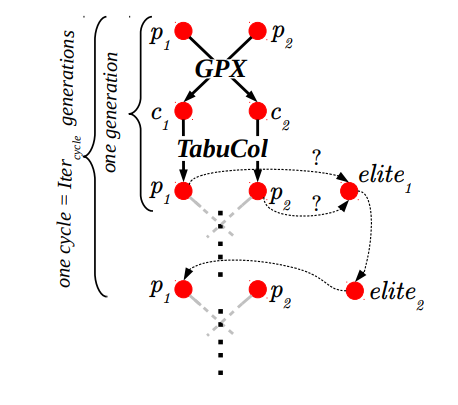
\includegraphics[scale=0.5]{head_algoritam}
\caption{Dijagram HEAD algoritma}
\label{head_algoritam}
\end{figure}

Naime, $elita_1$ predstavlja najbolje rešenje trentutne generacije, dok $elita_2$ najbolje rešenje prethodne. U svakoj iteraciji algoritma, jedna od novonastalih jedinki ukrštanjem zamenjuje se sa $elita_2$ jedinkom. Pretpostavka je da $elita_2$ se dovoljno razlikuje od jedinki trenutne generacije, i samim tim da doprinosi diverzifikaciji populacije.




\subsection{Problem trgovačkog putnika}
\label{sec:trgovacki_putnik}

TODO
















\subsection{Problem prepoznavanja zajednica}
\label{sec:prepoznavanje_zajednica}

TODO












\section{Zaključak}
\label{sec:zakljucak}

TODO

\addcontentsline{toc}{section}{Literatura}
\appendix
\bibliography{seminarski} 
\bibliographystyle{plain}

\appendix
\section{Dodatak}
TODO


\end{document}
